%%%%%%%%%%  scan idx 104  |  folio 91  %%%%%%%%%%
\SGAPrintPage{91}%
that the finiteness hypothesis on \(\Ho^n(G)\) is preserved; a new local correction in degree \(n\) then allows us to make \(\Ho^n(u)\) surjective.

The exact cohomology sequence
\[
  \longrightarrow \Ho^n(G)\longrightarrow
  \Ho^{n+1}(E)\longrightarrow
  \Ho^{n+1}(F)\longrightarrow
\]
shows that the kernel of \(\Ho^{n+1}(u)\) is of \(\underline{C}_0\)-finite type. In other words, the set of \(X\) over \(S\) such that there exists an exact sequence
\[
  M\longrightarrow \Ho^{n+1}(E_X)
  \xrightarrow{\Ho^{n+1}(u)}
  \Ho^{n+1}(F_X),
\]
with \(M\in\Ob\underline{C}_{0X}\), is a refinement of \(S\). Since \(\underline{C}_0\) is locally quasi-liftable in \(\underline{C}\), we can moreover require the arrow \(M\longrightarrow \Ho^{n+1}(E_X)\) to factor through \(Z^{n+1}(E_X)\) as
\[
  M\xrightarrow{r}Z^{n+1}(E_X)\longrightarrow \Ho^{n+1}(E_X).
\]
The composite arrow
\[
  M\xrightarrow{u_X^{n+1}r}Z^{n+1}(F_X)\longrightarrow \Ho^{n+1}(F_X)
\]
is zero by construction, so \(u_X^{n+1}r\) factors through \(B^{n+1}(F_X)=\operatorname{Im}\!\left(F_X^n\xrightarrow{d^n}F_X^{n+1}\right)\). Applying quasi-liftability again, we can require \(u_X^{n+1}r\) to factor through \(F_X^n\) as
\[
  M\xrightarrow{s}F_X^n\longrightarrow B^{n+1}(F_X)\longrightarrow Z^{n+1}(F_X).
\]
We then check trivially that \(u'\), defined as in (1.4.1), is a morphism of complexes satisfying (i).

Let \(G'\) be the cone of \(u':E'\to F_X\). Let us show that \(\Ho^n(G')\) is of \(\underline{C}_0\)-finite type. By construction, there is an exact sequence
\[
  0\longrightarrow E_X\xrightarrow{v}E'\longrightarrow M[-n]\longrightarrow 0,
\]
%%%%%%%%%%  scan idx 105  |  folio 92  %%%%%%%%%%
\SGAPrintPage{92}%
with \(u'v=u_X\). To compare \(G_X\) and \(G'\), we can, for example, form the ``octahedron'' of \(\Kpx(\underline{C}_X)\)
\[
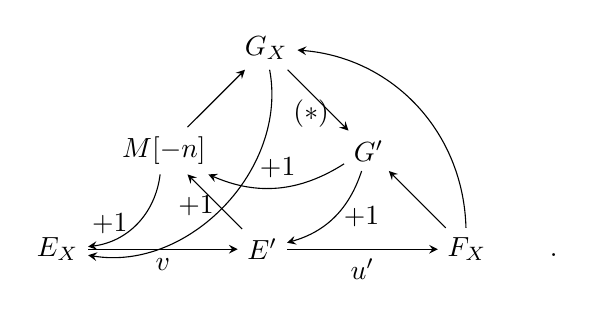
\begin{tikzpicture}[>=stealth,baseline=(GX.base),node distance=1.0cm]
  \node (EX) at (0,0) {$E_X$};
  \node (Ep) at (2.6,0) {$E'$};
  \node (FX) at (5.2,0) {$F_X$};
  \node (M)  at (1.35,1.25) {$M[-n]$};
  \node (GX) at (2.65,2.55) {$G_X$};
  \node (Gp) at (3.95,1.25) {$G'$};
  \node at (3.22,1.72) {$(*)$};
  \draw[->] (EX) -- node[below] {$v$} (Ep);
  \draw[->] (Ep) -- node[below] {$u'$} (FX);
  \draw[->] (Ep) -- (M);
  \draw[->] (M) -- (GX);
  \draw[->] (GX) -- (Gp);
  \draw[->] (FX) -- (Gp);
  \draw[->] (M) to[bend left=38] node[left] {$+1$} (EX);
  \draw[->] (Gp) to[bend left=28] node[above] {$+1$} (M);
  \draw[->] (Gp) to[bend left=28] node[right] {$+1$} (Ep);
  \draw[->] (GX) to[bend left=55] node[left] {$+1$} (EX);
  \draw[->] (FX) to[bend right=42] (GX);
  \node[anchor=base] at (6.3,0 |- FX.base) {.};
\end{tikzpicture}
\]
The exact cohomology sequence of the distinguished triangle \((*)\) shows that \(\Ho^n(G_X)\longrightarrow \Ho^n(G')\) is an epimorphism, hence that \(\Ho^n(G')\) is indeed of \(\underline{C}_0\)-finite type.

The preceding correction therefore reduces us to the case where \(\Ho^{n+1}(u)\) is a monomorphism, which we shall now assume. The exact cohomology sequence of \(E\to F\to G\) then gives an exact sequence
\begin{equation}\tag{.}
  \Ho^n(E)\xrightarrow{\Ho^n(u)}
  \Ho^n(F)\longrightarrow \Ho^n(G)\longrightarrow 0.
\end{equation}
Since \(\Ho^n(G)\) is of \(\underline{C}_0\)-finite type, the set of \(X\) over \(S\) such that there exists an epimorphism \(M\longrightarrow \Ho^n(G_X)\) with \(M\in\Ob\underline{C}_{0X}\) is, by definition, a refinement of \(S\). Using the quasi-liftability of \(\underline{C}_0\) in \(\underline{C}\), we can require this epimorphism to factor through \(Z^n(F_X)\) as
\[
  M\xrightarrow{s}Z^n(F_X)\longrightarrow \Ho^n(F_X)\longrightarrow \Ho^n(G_X).
\]
It is clear that \(u'\), defined as in (1.4.1) with \((r=0)\), is a morphism of complexes and that \(\Ho^{n+1}(u')=\Ho^{n+1}(u_X)\). On the other hand, it follows immediately from the exact sequence (.) that
%%%%%%%%%%  scan idx 106  |  folio 93  %%%%%%%%%%
\SGAPrintPage{93}%
\[
  \Ho^n(u'):\Ho^n(E_X)\oplus M\longrightarrow \Ho^n(F_X)
\]
is an epimorphism. This completes the proof of (1.4.1).

\sgaStableTarget{sga6.e01.lem.1-4-2}\textbf{Lemma 1.4.2.} \uline{Let} \(\underline{C}\) \uline{be an abelian category,} \(u:E\to F\) \uline{a morphism of complexes of} \(\underline{C}\) \uline{(resp.\ an arrow of} \(\Dpx(\underline{C})\)\uline{),} \(G\) \uline{the cone of} \(u\)\uline{. Equivalent conditions for a given} \(n\in\mathbb Z\):
\begin{enumerate}[label=(\roman*)]
\item \(\Ho^i(G)=0\) \uline{for} \(i\geq n\);
\item \(\Ho^i(u)\) \uline{is an isomorphism for} \(i>n\) \uline{and an epimorphism for} \(i=n\).
\end{enumerate}
The proof follows immediately from the exact cohomology sequence.

\sgaStableTarget{sga6.e01.def.1-4-3}\textbf{Definition 1.4.3.} \uline{We shall say that} \(u\) \uline{is an} \(n\)-quasi-isomorphism (\uline{resp.\ an} \(n\)-isomorphism) \uline{when} \(u\) \uline{satisfies the equivalent conditions of (1.4.2).}

That being so, we deduce at once from (1.4.1) the

\sgaStableTarget{sga6.e01.cor.1-4-4}\textbf{Corollary 1.4.4.} \uline{Let} \(\underline{S},S,\underline{C},\underline{C}_0\) \uline{be as in (1.4.1). Let} \(u:E\to F\) \uline{be an} \((n+1)\)\uline{-quasi-isomorphism of complexes of} \(\underline{C}_S\) \uline{(}\(n\in\mathbb Z\) \uline{given) such that} \(\Ho^n(G)\) \uline{is of} \(\underline{C}_0\)\uline{-finite type. Then the set of} \(X\) \uline{over} \(S\) \uline{such that there exist} \((M,r,s)\) \uline{as in (1.4.1) such that} \(u'\) \uline{is an} \(n\)\uline{-quasi-isomorphism is a refinement of} \(S\)\uline{.}

In pictorial terms, using the finiteness condition on \(\Ho^n(G)\), we can locally ``gain one notch'', i.e.\ modify \(u\) locally in degree \(n\) by adding to \(E^n\) an object of \(\underline{C}_0\) so as to make \(u\) an \(n\)-quasi-isomorphism.

\sgaStableTarget{sga6.e01.cor.1-4-5}\textbf{Corollary 1.4.5.} \uline{Let} \(\underline{C}\) \uline{be an abelian category,} \(n\in\mathbb Z\)\uline{, and} \(u:E\to F\) \uline{an} \(n\)\uline{-quasi-isomorphism of complexes of} \(\underline{C}\)\uline{. There exists a commutative diagram of} \(\Cpx(\underline{C})\)
\[
\begin{tikzcd}
E \arrow[r,"v"] \arrow[d,"u"'] & E' \arrow[dl,"u'"]\\
F & ,
\end{tikzcd}
\]
%%%%%%%%%%  scan idx 107  |  folio 94  %%%%%%%%%%
\SGAPrintPage{94}%
\uline{where} \(u'\) \uline{is a quasi-isomorphism and} \(v\) \uline{a monomorphism inducing the identity in degree} \(\geq n\) (i.e.\ such that \(E'^i=E^i\) and \(v^i=\id(E^i)\) for \(i\geq n\)).

\uline{Proof.} Applying (1.4.4) in the case where \(\underline{S}\) is the punctual site and \(\underline{C}_0=\underline{C}\), we obtain a commutative triangle of \(\Cpx(\underline{C})\)
\[
\begin{tikzcd}
E \arrow[r,"v_{n-1}"] \arrow[d,"u"'] & E'_{\,n-1} \arrow[dl,"u'_{n-1}"]\\
F & ,
\end{tikzcd}
\]
where \(u'_{n-1}\) is an \((n-1)\)-quasi-isomorphism and \(v_{n-1}\) a monomorphism inducing the identity in degree \(\geq n\). Iterating the procedure, we find, for \(i\leq n-1\), a sequence of commutative triangles of \(\Cpx(\underline{C})\)
\[
\begin{tikzcd}
E'_i \arrow[r,"v_{i-1}"] \arrow[d,"u'_i"'] & E'_{\,i-1} \arrow[dl,"u'_{i-1}"]\\
F & ,
\end{tikzcd}
\]
where \(u'_i\) is an \(i\)-quasi-isomorphism and \(v_{i-1}\) a monomorphism inducing the identity in degree \(\geq i\). The corollary follows by passage to the limit. More precisely, denoting by \(d'_i\) the differential of \(E'_i\), we define \(E'\) by
\[
  E'^i=E^i,\quad d'^i=d^i\quad\text{for }i\geq n,
\]
and
\[
  E'^i=(E'_i)^i,\quad d'^i=(d'_i)^i\quad\text{for }i<n,
\]
then \(v\) and \(u'\) by
\[
  v^j=(v_i v_{i+1}\ldots v_{n-1})^j,\qquad u'^j=(u'_i)^j\qquad\text{for }i\leq j,
\]
and we check at once that \(E'\), \(v\), \(u'\) so defined answer the question.

%%%%%%%%%%  scan idx 108  |  folio 95  %%%%%%%%%%
\SGAPrintPage{95}%
In other words, briefly, we can extend an \(n\)-quasi-isomorphism to a quasi-isomorphism ``without changing anything given in degree \(\geq n\)''.

\sgaStableTarget{sga6.e01.sec.2}\section*{2. Pseudo-coherent complexes}

\sgaStableTarget{sga6.e01.para.2-0}2.0. In this section, \(\underline{S}\) denotes a site, \(S\) an object of \(\underline{S}\), \(\underline{C}\) a flat abelian \(\underline{S}\)-category (1.1), and \(\underline{C}_0\) a strictly full additive sub-\(\underline{S}\)-category of \(\underline{C}\). We assume that \(\underline{C}_0\) is locally quasi-stable under kernels of epimorphisms (1.2) and locally quasi-liftable in \(\underline{C}\) (1.2).

\sgaStableTarget{sga6.e01.def.2-1}\textbf{Definition 2.1.} \uline{Let} \(X\in\Ob \underline{S}\)\uline{,} \(E\) \uline{be a complex of} \(\underline{C}_X\)\uline{, and} \(n\in\mathbb Z\)\uline{. We shall say that} \(E\) \uline{is} strictly \(\underline{C}_0\)-\(n\)-pseudo-coherent (resp.\ \(\underline{C}_0\)-pseudo-coherent, resp.\ \(\underline{C}_0\)-perfect) \uline{when} \(E^i=0\) \uline{for} \(i\) \uline{sufficiently large and} \(E^i\in\Ob\underline{C}_{0X}\) \uline{for} \(i\geq n\) \uline{(resp.\ for every} \(i\)\uline{, resp.\ for every} \(i\) \uline{and} \(E^i=0\) \uline{for almost every} \(i\)\uline{).}

When there is no risk of confusion, we shall sometimes say ``strictly \(n\)-pseudo-coherent (resp\dots)'' instead of ``strictly \(\underline{C}_0\)-\(n\)-pseudo-coherent (resp\dots)''.

\sgaStableTarget{sga6.e01.lem.2-1-1}\textbf{Lemma 2.1.1.} \uline{Let} \(E\in\Ob\Cpx(\underline{C}_S)\) \uline{and} \(n\in\mathbb Z\)\uline{. When} \(E\) \uline{is strictly} \(n\)\uline{-pseudo-coherent and} \(\Ho^i(E)=0\) \uline{for} \(i>n\)\uline{, then} \(\Ho^n(E)\) \uline{is of finite type.}

\uline{Proof.} The sequence
\[
  0\longrightarrow Z^n(E)\longrightarrow E^n\longrightarrow E^{n+1}\longrightarrow\ldots\longrightarrow 0
\]
is exact and \(E^i\in\Ob\underline{C}_0\) for \(i\geq n\). Since \(\underline{C}_0\) is locally quasi-stable under kernels of epimorphisms, it follows that \(Z^n(E)\) is of finite type, hence so is \(\Ho^n(E)\), which is a quotient of it.

